\section{Zestaw:}
\subsection{Pierwszy}
\subsubsection{}
\begin{enumerate}
\item Sieć  krystaliczna, węzły sieci, proste sieciowe, płaszczyzny sieciowe, wskaźniki Millera (hkl), Komórka elementarna i  typy układów krystalograficznych
\item Operacje symetrii, grupy punktowe.
\item Sieć prosta a sieć odwrotna. Objętości komórki elementarnej w sieci odwrotnej. Odległości międzypłaszczyznowe. Strefy Brillouina.
\end{enumerate}
\subsubsection*{Rozwiązanie:}


\subsubsection{}
Obliczyć objętość komórki elementarnej dla układu regularnego, romboedrycznego, heksagonalnego, jednoskośnego.
\subsubsection*{Rozwiązanie:}

\subsubsection{}
Wykaż, że:
\begin{enumerate}
\item dla prostej sieci regularnej o stałej sieciowej $a$, odległość międzypłaszczyznowa \[d^2_{hkl} =\frac{a^2}{h^2+k^2+l^2}\] 
\item obliczyć $\frac{1}{d^2_{hkl}}$ dla układu heksagonalnego oraz rombowego
\end{enumerate}
\subsubsection*{Rozwiązanie:}

\subsubsection{}
Struktura diamentu zawiera dwa identyczne atomy w położeniach $000$ i $\frac{1}{4}\frac{1}{4}\frac{1}{4}$ związane z każdym węzłem sieci powierzchniowo centrowanej \textit{(fcc)}. Obliczyć czynnik strukturalny dla tej struktury. Pokaż, że dozwolone odbicia spełniają warunek $h + k + l = 4n$, gdzie wszystkie wskaźniki są parzyste, a $n$ jest dowolna liczbą całkowitą, albo wszystkie składniki są nieparzyste.  
\subsubsection*{Rozwiązanie:}

\newpage

\subsection{Drugi}
\subsubsection{}
Energia oddziaływania między dwoma atomami w cząsteczce opisywana jest wzorem:
\[U(r) = -\frac{\alpha}{r^n}+\frac{\beta}{r^m}\]
Pokazać, że $m>n$.
\subsubsection*{Rozwiązanie:}
pierwsza pochodna:
\begin{equation}
\frac{\partial U}{\partial r} = \frac{n\alpha}{r^{n+1}} - \frac{m\beta}{r^{m+1}}=0 \rightarrow \frac{n\alpha}{r^{n+1}} = \frac{m\beta}{r^{m+1}}
\end{equation}
\begin{equation}
\label{eq:pp}
\frac{r^{m+1}}{r^{n+1}} = r^{m-n} = \frac{m\beta}{n\alpha}
\end{equation}
druga pochodna:
\begin{equation}
\frac{\partial^2 U}{\partial r^2} = - \frac{n(n+1)\alpha}{r^{n+2}} + \frac{m(m+1)\beta}{r^{m+2}} > 0
\end{equation}
\[ \frac{n(n+1)\alpha}{r^{n+2}} < \frac{m(m+1)\beta}{r^{m+2}} \]
\[n(n+1)\alpha \left( \frac{r^{m+2}}{r^{n+2}} \right) = n(n+1)\alpha r^{m-n} < m(m+1)\beta\]
z (\ref{eq:pp}):
\[ n(n+1)\alpha \frac{m\beta}{n\alpha} = (n+1)m\beta = nm\beta + m\beta < m^2\beta + m\beta\]
\[nm < m^2 \rightarrow n<m\]
\hrulefill

\subsubsection{}
Rozważ liniowy układ $2N$ jonów o ładunku równym na przemian $\pm q$. Załóż, że energia potencjalna odpychania między najbliższymi sąsiadami ma postać $\frac{A}{R^n}$. 
\begin{enumerate}
\item Pokaż, że dla odległości między jonami odpowiadającej stanowi równowagi 
\[U(R_0) = -\frac{2Nq^2\ln(2)}{R_0}\left(1-\frac{1}{n}\right)\]
\item Załóżmy, że kryształ został ściśnięty tak, że $R_0\rightarrow R_0(1-\delta)$. Pokaż, że w wyrażeniu na pracę związaną ze ściśnięciem kryształu największy wkład opisuje człon $\frac{C\delta^2}{2}$ gdzie:
\[C=\frac{(n-1)q^2\ln(2)}{R_0}\]
\end{enumerate}
\subsubsection*{Rozwiązanie:}
\begin{enumerate}
\item Energia potencjalna oddziaływania między dwoma atomami dana jest przez:
\begin{equation}
\label{eq:UR}
U(R) = N\left( \frac{A}{R^n} - \frac{\alpha q^2}{R} \right)
\end{equation}
gdzie $\alpha$ jest stałą Madelunga wynoszącą dla przypadku liniowego $\alpha = 2\ln 2$.\\
Dla stanu równowagi spełniony musi być warunek:
\begin{equation}
\frac{\partial U}{\partial R} = 0
\end{equation}
stąd:
\begin{equation}
\frac{\partial U}{\partial R} = N \left( -\frac{nA}{R_0^{n+1}} + \frac{\alpha q^2}{R_0^2} \right)= 0
\end{equation}
\begin{equation}
\label{eq:dudr}
\frac{nA}{R_0^{n+1}} = \frac{\alpha q^2}{R_0^2} \rightarrow \frac{A}{R_0^n} = \frac{\alpha q^2}{n R_0}
\end{equation}
Wstawiając wyrażenie (\ref{eq:dudr}) do (\ref{eq:UR}) oraz $\alpha=2\ln(2)$ otrzymuje się:
\begin{equation}
U(R_0) = N \left( \frac{\alpha q^2}{R_0^n} - \frac{\alpha q^2}{R_0} \right) = \frac{2Nq^2\ln(2)}{R_0} \left( \frac{1}{n} -1 \right)
\end{equation}
\hrulefill
\item yyy
\end{enumerate}

\subsubsection{}
Obliczyć stałą Madelunga dla kryształu \textit{NaCl}:
\begin{enumerate}
\item przypadek jednowymiarowy (nić krystaliczna \textit{NaCl})
\begin{figure}[h!]
\centering
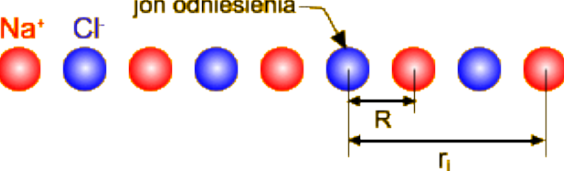
\includegraphics[scale=0.3]{images/zes2-1}
\end{figure}
\item przypadek dwuwymiarowy (siatka płaska \textit{NaCl})
\begin{figure}[h!]
\centering
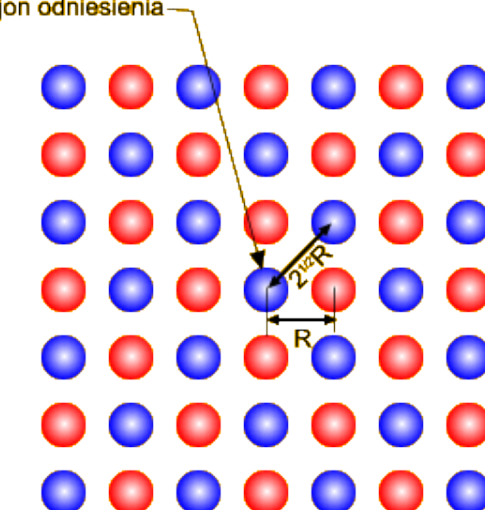
\includegraphics[scale=0.2]{images/zes2-2}
\end{figure}
\end{enumerate}
\subsubsection*{Rozwiązanie:}
\textbf{przypadek 1}
Stała Madelunga jest używana do wyznaczania potencjału elektrostatycznego pojedynczych jonów w krysztale, przez zbliżanie się jonów przez ładunki punktowe. 
\\
\\
wzór ogólny:
\\
\\
\begin{equation}
\alpha=\sum \frac {\pm}{p_i}
\end{equation}
\\
\\
W naszym przypadku: 
\\
\\
\begin{equation}
\frac{\alpha}{R}=2\left( \frac{1}{R}-\frac{1}{2R}+\frac{1}{3R}-\frac{1}{4R}+\frac{1}{5R} \right)
\end{equation}
\\
gdzie jako jon odniesienia bierzemy jon zaznaczony na rysunku, następnie odejmujemu lub dodajemy w zależności od znaku jonu w minaowniku są wielokrotności odległości od jonu odniesienia.
\\
\\
Używając rozwinięcia w szereg Maclurina możemy udowodnić, że szereg:
\\
\\
\begin{equation}
x-\frac{x^2}{2}+\frac{x^3}{3}-\frac{x^4}{4}....
\end{equation}
\\
\\
którego wzór ogólny ma postać:
\\
\\
\begin{equation}
\sum_{n=1}^{\infty}\frac{(-1)^{n+1}}{n}x^n
\end{equation}
\\
\\
jest zbierzny do funkcji ln(1+x), gdzie x=1.
\\
\\
Rozwinięcie:
\\
\\
$f(x)=ln(x+1)$   =>   $f(0)=ln(1)=0$
\\
\\
$f'(x)=-\frac{1}{(x+1)^2}$   =>   $f(0)=-1$
\\
\\
$f''(x)=\frac{2}{(x+1)^3}$   =>   $f(0)=2$
\\
\\
$f'''(x)=-\frac{6}{(x+1)^5}$   =>   $f(0)=-6$
\\
\\
$=0+1*\frac{x}{1}-1*\frac{x^2}{2}+\frac{x^3}{6}-\frac{x^4}{4}$
\\
\\
ogólny wynik:
$\alpha=2ln2$
\\
\\
\textbf{przypadek drugi}
\\
\\
Odległości obliczmy w natępujący sposób:
\\
\\
-jako jon odniesienia bierzemy jon w środku.
\\
\\
-dzielimy przestrzeń na cztery kwadraty i wszystko liczmy dla jednego kwadratu potem mnożymy razy cztery.
\\
\\
-pierwsze trzy wartości w nawiasie są to odległości od jonu odniesienia w prawo (liczmy je tak jak poprzednio, w liczniku znak, a wmianowniku wielokrotność odległości od jonu odniesienia)
\\
\\
-następnie liczmy odległość jonu oznaczone gwiazdką, mnożymy przez odpowiedni znak i dodajemy do sumy (liczmy ze wzoru Pitagorasa)
\\
\\
następnie liczmy odległości dwóch jonów oznaczonych paprykami i mnożymy razy dwa ponieważ na prawo od jonu z gwiazdką też mamy papryki.
\\
\\
-potem liczymy jony oznaczone słońcami 
\\
\\
-a na końcu jon oznaczony prostokątem i mnożymy razy dwa bo po prawej też jest prostokąt.
\\
\\
I wychodzi nam:
\\
\\
\begin{equation}
\frac{\alpha}{R} =\frac{4}{R}(1-\frac{1}{2}+\frac{1}{3}-\frac{1}{\sqrt{2}}=\frac{2}{\sqrt{5}}-\frac{2}{\sqrt{10}}-\frac{1}{2\sqrt{2}}-\frac{1}{3\sqrt{2}}+\frac{2}{\sqrt{13}})
\end{equation}
\\
\\
opisane wyżej odległości, które znajdują się w licznikach liczymy ze wzoru pitagorasa, np. dla jonu z gwiazdką:
\\
\\
\begin{equation}
R^2+R^2=R^2
\end{equation}
\begin{equation}
2R^2=R^2
\end{equation}
\begin{equation}
R=\sqrt{2}R
\end{equation}

\subsubsection{}
Obliczyć jakie ciśnienie należy przyłożyć do kryształu jonowego, aby odległość między jonami zmniejszyła się o $1$ procent.
\subsubsection*{Rozwiązanie:}
